En la quinta clase del curso, trabajaremos con clasificaci\'on no supervisada
de im\'agenes satelitales. Son nuestros objetivos:

\begin{itemize}
  \item Usar la herramienta de clasificaci\'on no supervisada.
  \item Aprender a indentificar clases espectrales en categor\'ias de uso y cobertura.
  \item Incorporar informaci\'on no espectral a las clasificaciones como
  pueden ser datos temporales o informaci\'on espacial.
  \item Aplicar la transformada por componentes principales para reducir la dimensionalidad
  y seleccionar los datos mas relevantes previos a las clasificaciones.
\end{itemize}

\section{Clasificaci\'on mediante el m\'etodo k-means}

Cargaremos primero la imagen Landsat 8 y habilitaremos la opci\'on para escribir
el header de ENVI\@.

\begin{lstlisting}
    rasterOptions(addheader = "ENVI")
    xml.2016 <- readMeta("raster_data/LC82240782016304/LC82240782016304LGN00.xml")
    ref.2016 <- stackMeta(xml.2016, quantity = "sre")
    scaleF <- getMeta(ref.2016,xml.2016, what = "SCALE_FACTOR")
    ref.2016 <- ref.2016 * scaleF
    ref.2016 <- ref.2016[[-1,]]
    names(ref.2016) <- c("blue","green","red","nir","swir1","swir2")
\end{lstlisting}

Veamos como clasificar una imagen usando el m\'etodo k-means en R. Vamos a usar
los paquetes \texttt{raster} y \texttt{RStoolbox}

\begin{exa}
    Elegimos la semilla para el geneador de n\'umeros aleatorios con el comando \texttt{set.seed(42)}. De esta forma la serie de n\'umeros aleatorios
    es la misma para todos.

    Luego clasificamos la imagen y la guardamos como vimos en las clases anteriores.

    \begin{lstlisting}
    set.seed(42)
    kmeans.2016 <- unsuperClass(ref.2016, nClasses = 5, nStarts = 100,
                                nSamples = 100)
    writeRaster(kmeans.2016$map, "raster_data/processed/kmeans2016",
                datatype="INT1U")
    \end{lstlisting}

    En este caso estamos solamente usando 5 clases espectrales. Podemos ahora graficar por separado cada una de las clases (figura \ref{fig:clases5}).

    \begin{lstlisting}
        clases.2016 <- layerize(kmeans.2016$map)
        plot(clases.2016)
    \end{lstlisting}

    \begin{figure}[h!]
      \centering
      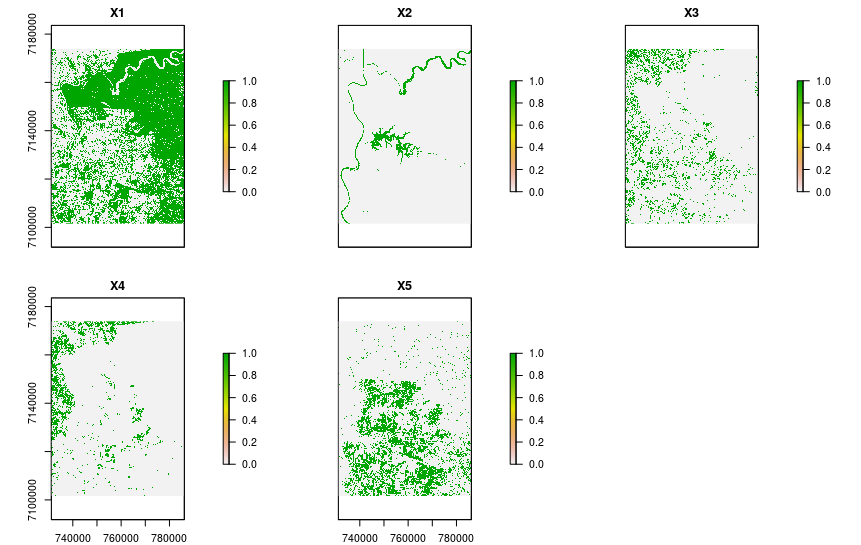
\includegraphics[width=0.7\textwidth]{clases_5.png}
      \caption{Clases generadas por el algoritmo kmeans para 5 clases.}
      \label{fig:clases5}
    \end{figure}

    Abriremos la imagen ahora en el QGIS e identificaremos cada una de las clases.

    Para realizar la identificacion primero vamos al men\'u \menu{propiedades de la imagen, Estilo, Tipo de renderizacion, Unibanda pseudocolor}. Elegimos de modo \menu{Intervalo Igual} y en n\'umero de clases ponemos con el m\'inimo en 1 y el m\'aximo en 5. En estilo de color elegimos colores aleatorios. Iremos luego cambiando los colores uno a uno por un color brillante e identificado a que cobertura pertenece dicha clase espectral.

    Construimos una tabla como la siguiente en un editor de texto.

    \begin{verbatim}
        id  class
        1   2
        2   7
        3   1
        4   1
        5   1
    \end{verbatim}

  La guardamos en un archivo de texto con el nombre \file{class.txt}.

  Una vez conocidas las categor\'ias de uso y cobertura correspondientes a cada
  clase espectral podemos combinarlas

  \begin{lstlisting}
      clases.2016 <- read.delim("aux_data/class.txt")
      reclas.2016 <- subs(kmeans.2016$map, clases.2016)
  \end{lstlisting}

  y graficarlas (figura \ref{fig:kmeans5})

  \begin{lstlisting}
    colores = c('#b2df8a','#33a02c',
                '#fdbf6f','#ff7f00',
                '#fb9a99','#e31a1c',
                '#a6cee3','#1f78b4')
    plot(reclas.2016, col=colores, zlim=c(1,8))
  \end{lstlisting}
  \begin{figure}[h!]
    \centering
    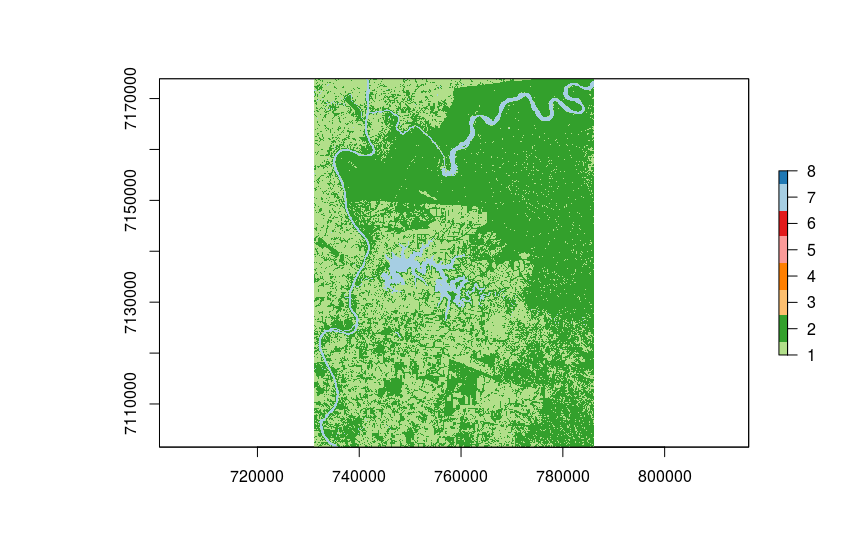
\includegraphics[width=0.7\textwidth]{kmeans-colores.png}
    \caption{Imagen clasificada por el m\'etodo kmeans con 5 clases espectraales.}
    \label{fig:kmean5}
  \end{figure}
\end{exa}

\begin{exa}
  Hagamos un an\'alisis espectral de las im\'agenes clasificadas antes y despues de la fusi\'on.  Para esto utilizaremos a la imagen clasificada como mascara para asignar los colores  al scatterplot.

  Agregamos la imagen clasificada a las bandas de la imagen en reflectancia y luego hacemos los scatterplot segun la clase espectral o de informaci\'on como

  \begin{lstlisting}
    stack.2016 <- stack(ref.2016, reclas.2016)
    xyplot(nir+swir1~red, groups=MC_ID, data=stack.2016)
  \end{lstlisting}

  Vemos que las clases espectrales pueden unirse en clases de informaci\'on y que algunas clases de informaci\'on no se separan en distintas clases espectrales (figuras \ref{fig:esk}).

  \begin{figure}[h!]
    \centering
    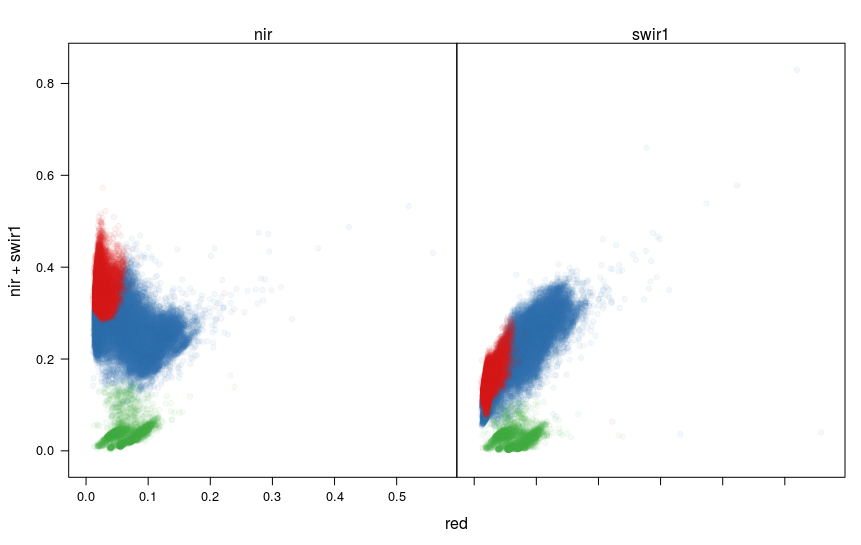
\includegraphics[width=0.7\textwidth]{kmeans-es.png}
    \caption{Espacio espectral clasificado por kmeans.}
    \label{fig:esk}
  \end{figure}

\end{exa}

\begin{exa}
  Repitamos este an\'alisis pero con 100 clases espectrales. El algor\'itmo es el mismo pero ahora vamos a usar el parametro \texttt{nClasses} igual a 100.

  \begin{lstlisting}
  set.seed(42)
  kmeans.2016b <- unsuperClass(ref.2016, nClasses = 100, nStarts = 100,
                              nSamples = 1000)
  writeRaster(kmeans.2016b$map, "raster_data/processed/kmeans2016b",
              datatype="INT1U", overwrite=TRUE)
  clasesb.2016 <- read.delim("aux_data/class100.txt")
  reclasb.2016 <- subs(kmeans.2016b$map, clasesb.2016)
  plot(reclasb.2016, col=colores, zlim=c(1,8))
  \end{lstlisting}

  Comparamos las classificacion obtenidas con 5 y 100 classes espectrales (figura \ref{fig:5v100})

  \begin{figure}[h!]
    \centering
    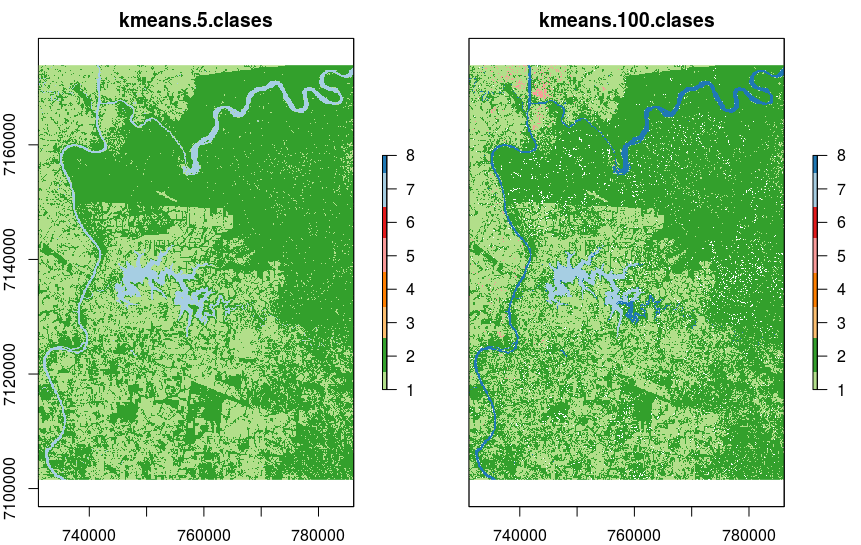
\includegraphics[width=0.7\textwidth]{5v100.png}
    \caption{Comparaci\'on entre la clasificaci\'on con 5 clases y 100 clases espectrales.}
    \label{fig:5v100}
  \end{figure}

  Comparamos nuevamente los espacios de fase entre la clasificacion obtenida a partir de 5 y 100 clases espectrales
  \begin{lstlisting}
    stackb.2016 <- stack(ref.2016, reclasb.2016)
    xyplot(nir+swir1~red, groups=MC_ID, data=stack.2016)
    xyplot(nir+swir1~red, groups=MC_ID, data=stackb.2016)
  \end{lstlisting}

\end{exa}

\begin{act}
  Repita la clasificaci\'on para la imagen landsat 7 del año 2000.
\end{act}


\section{Informacion espacial y temporal}

Con el fin de mejorar la clasificaci\'on podemos incorporar informaci\'on espacial y temporal a la informaci\'on radiom\'etrica. De esta forma estaremos, al momento de clasificar los p\'ixeles, ya no trabajando en un espacio espectral sino en uno mças amplio. Veamos como hacer esto.

\begin{exa}
  Para incorporar informacion espacial sobre el contexto del p\'ixel, podemos
  hacerlo tanto antes como despu\'es de la clasificaci\'on. Nos centraremos
  en este caso en como hacerlo antes.

  Calculamos primero la variabilidad local de brillo para la banda pancrom\'atica de la imagen Landsat 8 como

  \begin{lstlisting}
    pan.2016 <- raster("raster_data/LC82240782016304LGN00/LC82240782016304LGN00_B8.TIF")
    window <- matrix(1,nrow=5, ncol=5)
    sd.2016<-focal(pan.2016,w=window,fun=sd)
    plot(log(sd.2016,base = 10), zlim=c(1,4))
  \end{lstlisting}

  Vemos que las zonas con mayor presencia de urbanizaciones presentan una mayor variabilidad que aquellas con menor presencia (ver figura \ref{fig:pansd}).

  \begin{figure}[h!]
    \centering
    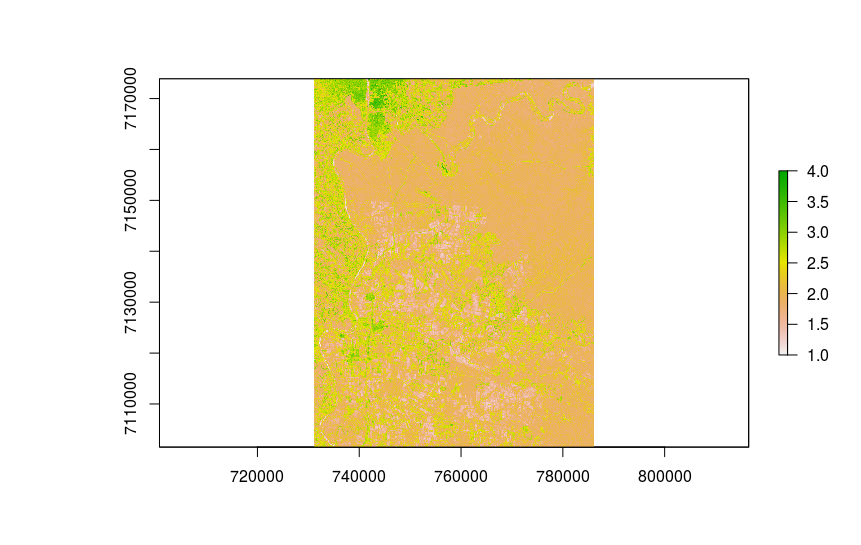
\includegraphics[width=0.7\textwidth]{pan-sd.png}
    \caption{Desv\'io standar para una ventana de 5 p\'ixeles por 5 p\'ixeles en escala logar\'itmica.}
    \label{fig:pansd}
  \end{figure}

  Una vez obtenida la banda de desvio standar, podemos agregarla a las demas, luego de remuestrearla haciendo

  \begin{lstlisting}
    sd.2016 <- aggregate(sd.2016, fact=2, fun=mean)
    stack(ref.2016, sd.2016)
    pca.2016 <- rasterPCA(stack(ref.2016, sd.2016), spca = TRUE)
  \end{lstlisting}

  \begin{Verbatim}[fontsize=\small]
  Importance of components:
                            Comp.1    Comp.2    Comp.3     Comp.4      Comp.5 ...
  Standard deviation     2.1592402 1.1821570 0.8392878 0.40888073 0.196591748 ...
  Proportion of Variance 0.6660455 0.1996422 0.1006292 0.02388335 0.005521188 ...
  Cumulative Proportion  0.6660455 0.8656876 0.9663168 0.99020013 0.995721318 ...
  \end{Verbatim}

  Vemos en este caso, analizando el sumario, que la banda de textura agrega informaci\'on con respecto a la s\'olo disponible al utilizar las bandas en reflectancia.
\end{exa}

\begin{act}
  Repita el ejemplo para la imagen landsat 7 del año 2000. Clasifique por el metodo de kmeans las imagenes de los años 2000 y 2016.
\end{act}

\begin{exa}
  Para incorporar informacion del contexto temporal, agregaremos a la informaci\'on espectral informaci\'on sobre la variaci\'on del \'indice de vegetaci\'on durante el año en que se tomo la imagen. Primero cargamos las im\'agenes MODIS del 2016

  \begin{lstlisting}
    list.2016 <- list.files("raster_data/MOD13Q1/NDVI/", pattern = "MOD13Q1.A2016+.*tif", full.names = TRUE)
    ndvi.2016 <- stack(list.2016)/1e4
    ndvi.2016 <- approxNA(ndvi.2016)
    sd.2016 <- calc(ndvi.2016, fun = sd)
    me.2016 <- calc(ndvi.2016, fun = mean)
    plot(stack(me.2016,sd.2016))
  \end{lstlisting}

  Una vez hecho esto, resampleamos el promedio y el desv\'io de la serie temporal y lo unimos a las im\'agenes en reflectancia, sobre las cuales calcularemos la transformada por componentes principales.

  \begin{lstlisting}
    sd.2016 <- resample(sd.2016, ref.2016, method="ngb")
    me.2016 <- resample(me.2016, ref.2016, method="ngb")
    pca.2016 <- rasterPCA(stack(ref.2016, me.2016, sd.2016), spca = TRUE)
    summary(pca.2016$model)
  \end{lstlisting}
\end{exa}

\begin{act}
  Repita el ejemplo para la imagen Landsat 7 del año 2000. Clasifique por el metodo de kmeans las imagenes de los años 2000 y 2016.
\end{act}
